\documentclass[tikz,10pt]{standalone}
\usepackage{amsmath,amssymb,cmap,pgfplots,pgfplotstable}
\usetikzlibrary{arrows,calc,intersections}
\pgfplotsset{compat=newest}

\begin{document} 
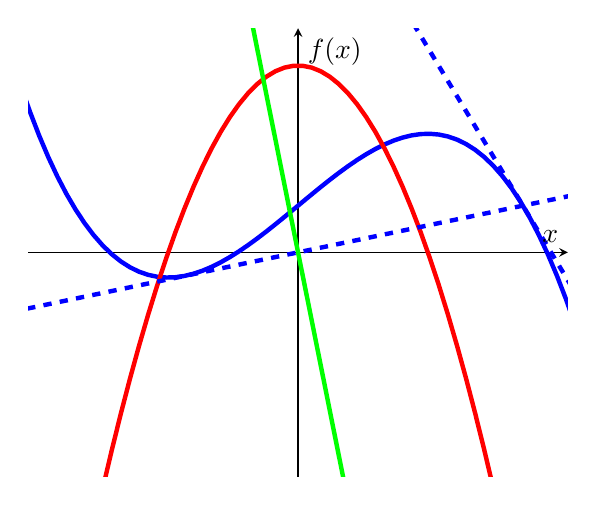
\begin{tikzpicture}
\begin{axis}[
xlabel={$x$},
ylabel={$f(x)$},
axis lines=middle,
ymax = 1,
ymin = -1,
xmax = 1,
xmin = -1,
enlargelimits=true,
%restrict y to domain=-200:200,
xtick=\empty,
ytick=\empty
]
\addplot[
blue!,
line width=1.6pt,
domain={-2:2},
samples=100
]{-x^3 + x + 0.25};
\addplot[
red!,
line width=1.6pt,
domain={-2:2},
samples=100
]{-3*x^2+1};
\addplot[
green!,
line width=1.6pt,
domain={-2:2},
samples=100
]{-6*x};
\addplot[
blue!,
dashed,
line width=1.6pt,
domain={-2:2},
samples=100
]{-2*x+2.25};
\addplot[
blue!,
dashed,
line width=1.6pt,
domain={-2:2},
samples=100
]{0.25*x};
\end{axis}
\end{tikzpicture}\end{document}